\subsection{Vyjádření přímky pomocí dvou rovnic}
\label{subsec:Line_in_space_as_intersection_of_planes}

V rovině jsme přímku dokázali popsat jedinou obecnou rovnicí
\[
    ax+by+c=0.
\]
V prostoru však obdobná lineární rovnice
\[
    ax+by+cz+d=0
\]
obecně nepopisuje přímku, ale rovinu. \textbf{Obecná rovnice přímky
v prostoru proto neexistuje.}
Přímku v prostoru lze přesto pomocí lineárních rovnic vyjádřit. Potřebujeme
k tomu zpravidla dvě rovnice, z nichž každá určuje jednu rovinu. Jestliže
se tyto roviny protínají, je jejich průnikem přímka, kterou nazýváme
\textbf{průsečnicí rovin}.

Přímku $p$ tak můžeme zapsat ve tvaru
\[
    p:\quad
    \begin{cases}
        a_1x+b_1y+c_1z+d_1=0,\\
        a_2x+b_2y+c_2z+d_2=0.
    \end{cases}
\]
Tento zápis však není obecnou rovnicí přímky. Jde o soustavu dvou rovnic,
která vyjadřuje přímku jako společnou část dvou rovin.

Nejjednodušším příkladem je osa $z$. Všechny její body mají nulovou
$x$-ovou a $y$-ovou souřadnici, a proto ji můžeme zapsat jako
\[
    p:\quad
    \begin{cases}
        x=0,\\
        y=0.
    \end{cases}
\]
Rovnice $x=0$ určuje souřadnicovou rovinu $yz$ a rovnice $y=0$ určuje
souřadnicovou rovinu $xz$. Jejich průsečnicí je právě osa $z$.

\begin{figure}[H]
    \centering
    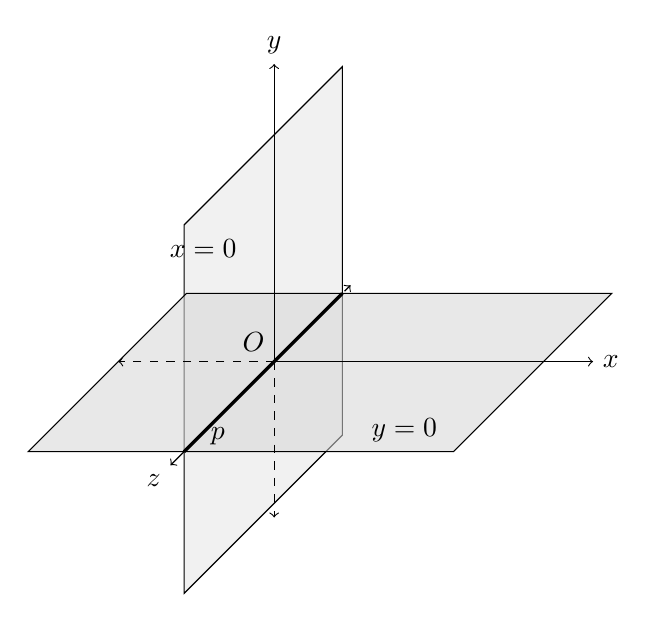
\begin{tikzpicture}[scale=0.9]

        % Rovina yz: x = 0
        \fill[gray!15, fill opacity=0.75]
            (0,-2,-2.5) -- (0,3.2,-2.5) --
            (0,3.2,3.3) -- (0,-2,3.3) -- cycle;
        \draw[thin]
            (0,-2,-2.5) -- (0,3.2,-2.5) --
            (0,3.2,3.3) -- (0,-2,3.3) -- cycle;

        % Rovina xz: y = 0
        \fill[gray!32, fill opacity=0.55]
            (-2.2,0,-2.5) -- (3.8,0,-2.5) --
            (3.8,0,3.3) -- (-2.2,0,3.3) -- cycle;
        \draw[thin]
            (-2.2,0,-2.5) -- (3.8,0,-2.5) --
            (3.8,0,3.3) -- (-2.2,0,3.3) -- cycle;

        % Osy - kladná část
        \draw[->] (0,0,0) -- (4.5,0,0) node[right] {$x$};
        \draw[->] (0,0,0) -- (0,4.2,0) node[above] {$y$};
        \draw[->] (0,0,0) -- (0,0,3.8) node[below left] {$z$};

        % Osy - záporná část
        \draw[->, dashed] (0,0,0) -- (-2.2,0,0);
        \draw[->, dashed] (0,0,0) -- (0,-2.2,0);
        \draw[->, dashed] (0,0,0) -- (0,0,-2.8);

        % Průsečnice rovin
        \draw[very thick] (0,0,-2.5) -- (0,0,3.3)
            node[pos=0.9, right] {$p$};

        \node[above left] at (0,0,0) {$O$};
        \node at (0,2.6,2.6) {$x=0$};
        \node at (2.8,0,2.5) {$y=0$};

    \end{tikzpicture}
    \caption{Osa $z$ je průsečnicí rovin $x=0$ a $y=0$.}
    \label{fig:Z_axis_as_intersection_of_planes}
\end{figure}

\begin{remark}
    Vyjádřením přímky jako průsečnice dvou rovin se nyní nebudeme
    podrobněji zabývat. Nejprve musíme poznat, jak lze roviny v prostoru
    popsat a jaké mohou mít vzájemné polohy. K tomuto způsobu vyjádření
    přímky se proto můžeme vrátit později.
\end{remark}

Tato úvaha nás přirozeně přivádí k dalšímu základnímu geometrickému
objektu v prostoru, kterým je rovina.
